\chapter{Θεωρητική Μελέτη των Μεθόδων}
\label{ch:chapter2}
\section{Μέθοδος Διχοτόμου}
Η μέθοδος Διχοτόμου ανήκει στις ακολουθιακές μεθόδους αναζήτησης. Το βασικό της χαρακτηριστικό είναι ότι σε κάθε βήμα, το διάστημα αναζήτησης $[\alpha, \beta]$ διαιρείται σε τρία υπό-διαστήματα, χωρισμένα από σημεία $x_1, x_2$ τοποθετημένα συμμετρικά σε απόσταση $\epsilon$ από την διχοτόμο του διαστήματος $[\alpha, \beta]$. Απορρίπτουμε το ένα από τα δύο μισά του διαστήματος και επαναλαμβάνουμε τη διαδικασία. Η διαδικασία επαναλαμβάνεται μέχρι να επιτευχθεί η επιθυμητή ακρίβεια $l$. Η απλή υλοποίηση της μεθόδου αποτελεί ίσως το μεγαλύτερο της πλεονέκτημα, όμως υστερεί όσον αφορά την ακρίβεια συγκριτικά με τις άλλες μεθόδους για μεγάλο αριθμό επαναλήψεων, ενώ απαιτεί να εκτιμηθεί η τάξη μεγέθους της συνάρτησης για την επιλογή της παραμέτρου $\epsilon$  

\begin{figure}[H]
    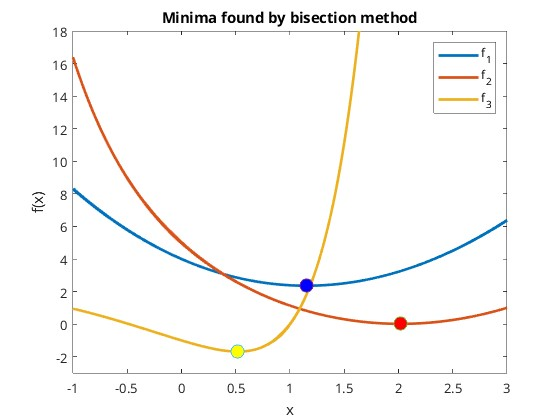
\includegraphics[scale=0.7]{plots/prereqs/bm.jpg}
    \label{fig:funcs}
    \caption{Τα ελάχιστα των συναρτήσεων με τη χρήση της Μεθόδου Διχοτόμησης}
    \centering
\end{figure}

\section{Μέθοδος Χρυσής Τομής}
Η μέθοδος της Χρυσής Τομής βασίζεται στη χρήση του αριθμού της Χρυσής Τομής $\phi = \frac{1 + \sqrt{5}}{2} \approx 1.618$. Σε κάθε βήμα της μεθόδου, δύο νέα σημεία $x_1, x_2$ δημιουργούνται στο διάστημα $[\alpha, \beta]$ με βάση τη Χρυσή Τομή. Αν $f(x_1) < f(x_2)$, τότε το σημείο ελαχίστου βρίσκεται στο $[\alpha, x_2]$, αλλιώς στο $[x_1, \beta]$. Με αυτή την επαναληπτική διαδικασία, το διάστημα μειώνεται κατά την αναλογία της Χρυσής Τομής σε κάθε βήμα. Το πλεονέκτημα της μεθόδου Χρυσής Τομής συγκριτικά με την Μέθοδο Διχοτόμου είναι ότι σε κάθε επανάληψη απαιτείται μονάχα ένας υπολογισμός της $f(x)$, καθώς οι υπολογισμοί της $f$ επαναχρησιμοποιούνται. Επίσης δεν χρειάζεται επιλογή της παραμέτρου $\epsilon$.

\begin{figure}[H]
    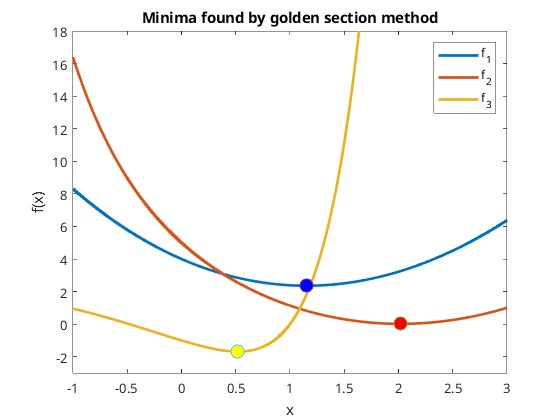
\includegraphics[scale=0.7]{plots/prereqs/gs.jpg}
    \label{fig:funcs}
    \caption{Τα ελάχιστα των συναρτήσεων με τη χρήση της Μεθόδου Χρυσής Τομής}
    \centering
\end{figure}

\section{Μέθοδος \selectlanguage{english} Fibonacci \selectlanguage{greek}}
Η βασική λογική της μεθόδου \selectlanguage{english}Fibonacci\selectlanguage{greek} είναι παρόμοια με της Χρυσής Τομής, αλλά η σύγκλιση του διαστήματος γίνεται σε προκαθορισμένα βήματα βάσει της ακολουθίας \selectlanguage{english}Fibonacci\selectlanguage{greek}, η οποία επιτρέπει την βελτιστοποίηση του αριθμού των υπολογισμών της συνάρτησης. Η Μέθοδος \selectlanguage{english}Fibonacci\selectlanguage{greek} προτιμάται σε περιπτώσεις που υπάρχει περιορισμένος αριθμός αξιολογίσεων της $f$, όμως η υλοποίηση της είναι πιο πολύπλοκη λόγω της απαίτησης επιλογής του αριθμού επαναλήψεων εκ των προτέρων.

\begin{figure}[H]
    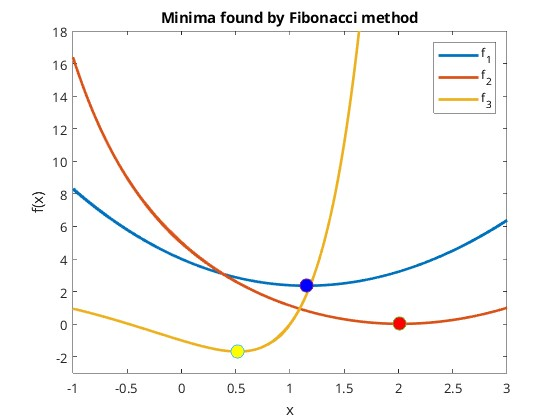
\includegraphics[scale=0.7]{plots/prereqs/fib.jpg}
    \label{fig:funcs}
    \caption{Τα ελάχιστα των συναρτήσεων με τη χρήση της Μεθόδου \selectlanguage{english} Fibonacci}\selectlanguage{greek}
    \centering
\end{figure}

\section{Μέθοδος Διχοτόμου με Χρήση Παραγώγων}
Η μέθοδος Διχοτόμου με χρήση παραγώγων είναι μια παραλλαγή της απλής Διχοτόμου που αξιοποιεί την πληροφορία της πρώτης παραγώγου της συνάρτησης. Ως αποτέλεσμα, λόγω της εκμετάλλευσης των πληροφοριών της παραγώγου, η μέθοδος μπορεί να είναι ταχύτερη από τη βασική Διχοτόμο χωρίς παράγωγο, ειδικά για προβλήματα όπου η παράγωγος είναι εύκολα υπολογίσιμη.

\begin{figure}[H]
    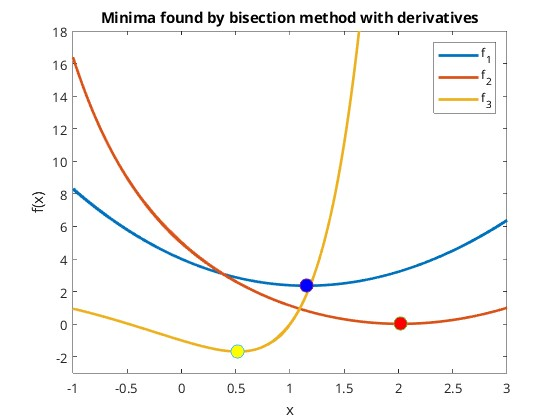
\includegraphics[scale=0.7]{plots/prereqs/bmd.jpg}
    \label{fig:funcs}
    \caption{Τα ελάχιστα των συναρτήσεων με τη χρήση της Μεθόδου Διχοτόμου με Χρήση Παραγώγων}
    \centering
\end{figure}